\begin{figure}[H]
    \centering
    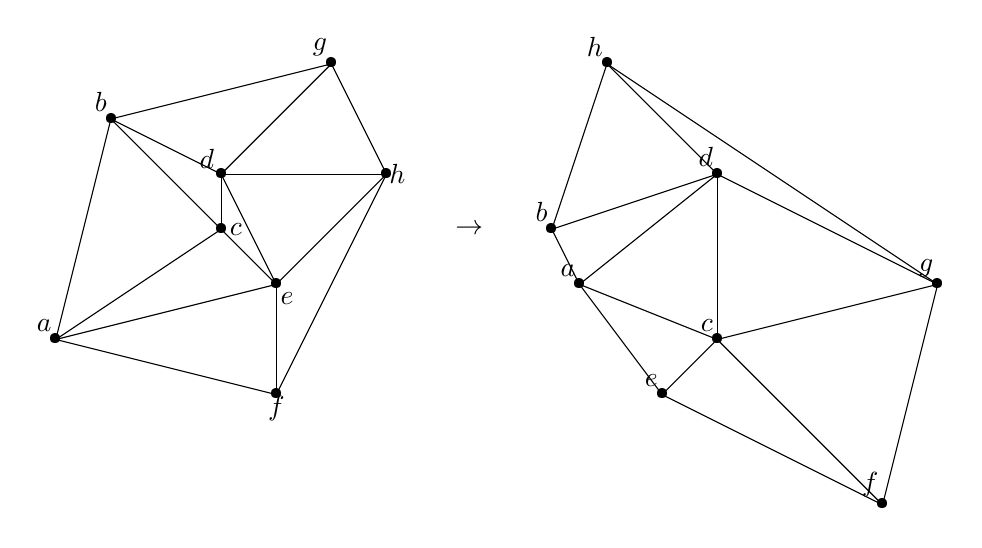
\begin{tikzpicture}[scale=0.7]
        \node[label={[label distance = -3mm]160:$a$}] at
        (-2.00, -1.00) {\textbullet};
        \node[label={[label distance = -3mm]160:$b$}] at
        (-1.00, 3.00) {\textbullet};
        \node[label={[label distance = -6mm]180:$c$}] at
        (1.00, 1.00) {\textbullet};
        \node[label={[label distance = -3mm]120:$d$}] at
        (1.00, 2.00) {\textbullet};
        \node[label={[label distance = -3mm]340:$e$}] at
        (2.00, 0.00) {\textbullet};
        \node[label={[label distance = -3mm]270:$f$}] at
        (2.00, -2.00) {\textbullet};
        \node[label={[label distance = -3mm]160:$g$}] at
        (3.00, 4.00) {\textbullet};
        \node[label={[label distance = -3mm]0:$h$}] at
        (4.00, 2.00) {\textbullet};

        \draw (-2.00, -1.00) -- (-1.00, 3.00); % a -- b
        \draw (-2.00, -1.00) -- (1.00, 1.00); % a -- c
        \draw (-2.00, -1.00) -- (2.00, 0.00); % a -- e
        \draw (-2.00, -1.00) -- (2.00, -2.00); % a -- f
        \draw (-1.00, 3.00) -- (1.00, 1.00); % b -- c
        \draw (-1.00, 3.00) -- (1.00, 2.00); % b -- d
        \draw (-1.00, 3.00) -- (3.00, 4.00); % b -- g
        \draw (1.00, 1.00) -- (1.00, 2.00); % c -- d
        \draw (1.00, 1.00) -- (2.00, 0.00); % c -- e
        \draw (1.00, 2.00) -- (2.00, 0.00); % d -- e
        \draw (1.00, 2.00) -- (3.00, 4.00); % d -- g
        \draw (1.00, 2.00) -- (4.00, 2.00); % d -- h
        \draw (2.00, 0.00) -- (2.00, -2.00); % e -- f
        \draw (2.00, 0.00) -- (4.00, 2.00); % e -- h
        \draw (2.00, -2.00) -- (4.00, 2.00); % f -- h
        \draw (3.00, 4.00) -- (4.00, 2.00); % g -- h

        \node at (5.5, 1.00) {$\rightarrow$};

        \begin{scope}
            [shift={(7, 0)}]
            \node[label={[label distance = -3mm]160:$a$}] at
            (0.5, 0) {\textbullet};
            \node[label={[label distance = -3mm]160:$b$}] at
            (0, 1) {\textbullet};
            \node[label={[label distance = -3mm]160:$c$}] at
            (3, -1) {\textbullet};
            \node[label={[label distance = -3mm]160:$d$}] at
            (3, 2) {\textbullet};
            \node[label={[label distance = -3mm]160:$e$}] at
            (2, -2) {\textbullet};
            \node[label={[label distance = -3mm]160:$f$}] at
            (6, -4) {\textbullet};
            \node[label={[label distance = -3mm]160:$g$}] at
            (7, 0) {\textbullet};
            \node[label={[label distance = -3mm]160:$h$}] at
            (1, 4) {\textbullet};

            \draw (0.5, 0) -- (0, 1); % a -- b
            \draw (0.5, 0) -- (3, -1); % a -- c
            \draw (0.5, 0) -- (3, 2); % a -- d
            \draw (0.5, 0) -- (2, -2); % a -- e
            \draw (0, 1) -- (3, 2); % b -- d
            \draw (0, 1) -- (1, 4); % b -- h
            \draw (3, -1) -- (3, 2); % c -- d
            \draw (3, -1) -- (2, -2); % c -- e
            \draw (3, -1) -- (6, -4); % c -- f
            \draw (3, -1) -- (7, 0); % c -- g
            \draw (3, 2) -- (7, 0); % d -- g
            \draw (3, 2) -- (1, 4); % d -- h
            \draw (2, -2) -- (6, -4); % e -- f
            \draw (6, -4) -- (7, 0); % f -- g
            \draw (7, 0) -- (1, 4); % g -- h
        \end{scope}
    \end{tikzpicture}
    \caption[Exemplo triangulação de Delaunay]{Triangulação de Delaunay da coleção de pontos nos instantes $t = 0$ e $t = 2$.}
    \label{fig:delaunay:exemplo}
\end{figure}